\chapterimage{./Pictures/cover-socket} % Chapter heading image
\chapter{TP7+TP8 : Communication socket}

\section{Communication distante en utilisant l’outil netcat}

\subsection{Exercice 1 : Découverte de la commande nc : netcat}
\textit{L’objectif de cet exercice est de nous familiariser avec une commande puissante appelée \mintinline{shell}{nc}. Cette commande, inspirée de la commande \mintinline{shell}{cat}, permet d’afficher et de recevoir un flux d’octets, non pas à l’écran et depuis le clavier, mais sur ou depuis le réseau, et plus précisément vers un processus distant identifié par une adresse ip un numéro de port et un mode (connecté "TCP" ou non connecté "UDP")}
\\\\
Afin de lancer un serveur TCP sur le port 3000 nous utilisons la commande \mintinline{shell}{nc -l 3000}. Elle affichera à l'écran tous les messages recu par le serveur.\\
Afin de lancer un client TCP qui se connectera au serveur TCP nous utilisons la commande \mintinline{shell}{nc localhost 3000}

\subsection{Exercice 2 : Utilisation de la commande nc : netcat pour le transfert de fichier et l’évaluation de la bande passante}
\textit{La commande netcat, souvent réduite au nom nc, est un utilitaire très puissant qui reprend le principe de la commande cat sur un support réseau. Les possibilités de cette commande sont énormes, et permettent de mettre en place très simplement un serveur en mode connecté ou non connecté pour transférer du texte ou un fichier. Cette commande peut également jouer le rôle de client.}
\\\\
Pour transférer un fichier il faut :
\begin{itemize}
  \item Coté émetteur : utiliser la commande \mintinline{shell}{nc <ip_address>:<port> > <filename>}
  \item Coté récepteur : utiliser la commande \mintinline{shell}{nc <ip_address>:<port> < <filename>}
\end{itemize}

La commande \mintinline{shell}{time} mise avant \mintinline{shell}{nc} nous pouvons avoir les informations de temps de transfert.\\
L'option verbose \mintinline{shell}{-v} permet d'activer le mode verbeux de la commande afin d'avoir des informations complémentaires.
\subsection{Exercice 3 : Une histoire de serveurs concurrents ...}
\textit{Dans cet exercice, nous regardons quelles capacités de cohabitation existent entre des serveurs qui voudraient utiliser le même port de communication}
\\\\
Il est possible de connecter plusieurs serveur tcp.
\begin{itemize}
  \item Le premier hôte se connectera au premier server TCP créé.
  \item Le deuxième hôte se connectera au deuxième server TCP créé.
  \item ainsi de suite.
\end{itemize}
Il en est de même pour la connexion de plusieurs serveurs UDP.
\\\\
Si nous souhaitons faire un montage avec un serveur tcp et un serveur udp, les clients tcp communiqueraient avec le serveur tcp et les clients udp avec les serveurs udp.\\
Il s'affichera un message d'erreur sur les serveur TCP \textit{Address already use}. Cela signifie que si nous nous connectons sur un port avec plusieurs serveurs nous discuterons avec les deux serveurs.

\subsection{Exercice 4 : Comprendre une requête HTTP}
\textit{Dans cet exercice, nous regardons une utilisation simple et originale de \mintinline{shell}{netcat} : comprendre ce que votre navigateur internet envoie comme information lorsqu’il effectue une requête sur un site web}
\\\\
Les protocoles de communication internet, comme le protocole \textbf{HTTP} (HyperTex Transfer Protocol) utilise communément le port 80 d'un client et d'un serveur pour envoyer et recevoir des données.
Après avoir démarrer une écoute local sur le port 80 à l'aide de la commande \mintinline{shell}{nc -l 80} nous pourront voir la console afficher les requetes HTTP.\\
À l'aide de notre navigateur internet nous pouvons nous connecter au serveur local à l'url \textit{http://localhost:80}.\\
Le navigateur nous indique que le site ne peut être atteint mais le serveur nous indique la requète transmise par le navigateur :

\begin{minted}{shell}
GET / HTTP/1.1
Host: localhost
Connection: keep-alive
Save-Data: on
User-Agent: Mozilla/5.0 (X11; Linux x86_64) AppleWebKit/537.36 (KHTML, like Gecko) Ubuntu Chromium/63.0.3239.132 Chrome/63.0.3239.132 Safari/537.36
Upgrade-Insecure-Requests: 1
Accept: text/html,application/xhtml+xml,application/xml;q=0.9,image/webp,image/apng,*/*;q=0.8
Accept-Encoding: gzip, deflate, br
Accept-Language: fr-FR,fr;q=0.9,en-US;q=0.8,en;q=0.7
\end{minted}

Plusieurs informations de la requête client peuvent être utile :
\begin{itemize}
  \item La ligne de requete comprennant la méthode (ici GET), l'URI (ici aucun) ainsi que la version HTTP (ici 1.1)
  \item L'entête de la requête contenant :
  \begin{itemize}
    \item Le type de connection (ici "keep-alive")
    \item L'url utilisé (ici localhost)
    \item Les données acceptés
    \item L'User-Agent : L'agent utilisé par le client pour envoyer la requete HTTP. Le navigateur internet (Chrome, Safari, Mozilla...) ainsi que le système d'exploitation (MacOS, Ubunutu, Windows ...).
  \end{itemize}
  \item d'autre données utiles peuvent être aussi présente comme la taille et le type du contenu, le corps de la requète ...
\end{itemize}

On remarque qu'en utilisant le protocle HTTPS (HTTP + Encryption -TCL/SSL) notre serveur recoit des données non exploitable puisqu'aucun contrat de cryptage entre les deux machines n'a été effectué.

\section{Développement d’un client et d’un serveur en C}
\subsection{Exercice 5 : Mise en place d’une communication en mode non connecte}
\textit{L’objectif de cet exercice est de découvrir les fonctions et structures de base en C permettant une communication en mode non connecté UDP.}
\\\\
Je propose le code ci-dessous afin d'implementer un client UDP ayant le comportement demandé :
\inputminted[linenos,firstline=30,lastline=91]{cpp}{../sources/cpp/TP7-8/clientUDP.c}

Je propose le code ci-dessous afin d'implementer un serveur UDP ayant le comportement demandé :
\inputminted[linenos,firstline=33,lastline=114]{cpp}{../sources/cpp/TP7-8/serveurUDP.c}

Après avoir lancé le serveur UDP nous testerons la communication entre le serveur UDP et le client UDP à l'aide de la commande \mintinline{bash}{UDClient <IP> <port> <message>} ainsi nous précisons au client l'IP et le port du serveur mais aussi le message que nous souhaitons envoyer.\\
\mintinline{shell}{UDClient 0.0.0.0 5000 "tset ysae"}\\
Le message reviens dans le même ordre "tset ysae".

\subsection{Exercice 6 : Création d’une architecture (client UDP) - (relai UDP-TCP) - (serveur TCP)}

\textit{L'objectif de cet exercice est de manipuler les deux mode (connecté et non connecté), en faisant communiquer un serveur tournant en TCP avec un client tournant en UDP. Cette communication n’est pas directement possible et nécessite un processus intermédiaire qui fera le relai entre le client et serveur.}
\\\\
À l'aide des instructions données dans le sujet de l'exercice et du code du serveur UDP nous pouvons implémenter le code principale d'un serveur TCP étant similaire à celui d'un serveur UDP. Le serveur TCP attend sur sa socket principale une connection et dès que une connection est accepté la connexion passe ensuite sur une socket de travail et écoute les données de cette dernière. Les données seront inversés avant de r'envoyer à son tour le message et termine la connection et retourne écouter la socket principale en attendant une autre connexion.\\
Le code implémenté est le suivant :
\inputminted[linenos, firstline=26,lastline=117]{cpp}{../sources/cpp/TP7-8/serveurTCP.c}

Le relai UDP TCP, se charge de transmettre le message communiqué par le client UDP, au serveur TCP et réciproquement, transmettre la réponse du serveur TCP au client UDP. Pour celà le relai doit utiliser le bon mode de communication (connecté ou non connecté) avec les deux entités.\\
Nous pouvons implémenter le code du relai UDP-TCP :
\inputminted[linenos, firstline=14,lastline=122]{cpp}{../sources/cpp/TP7-8/relaiUDPTCP.c}

Après avoir lancé le serveur TCP ainsi que le relai UDP-TCP nous testerons la communication entre le client UDP et le serveur TCP passant par le relai UDP-TCP à l'aide de la commande \mintinline{bash}{UDPClient <IP> <port> <message>} ainsi nous précisons au client l'IP et le port du serveur mais aussi le message que nous souhaitons envoyer.\\
\mintinline{shell}{UDClient 0.0.0.0 5000 "tset ysae"}\\
Le message reviens dans l'ordre inversé "easy test". Le serveur a donc effectué son travail et la communication est donc réussite.

\begin{figure}[H]
  \centering
  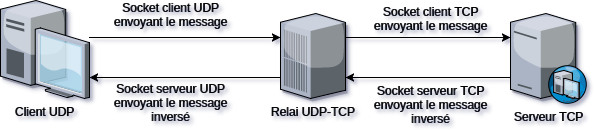
\includegraphics[width=300pt]{./cpp/Pictures/tp7+tp8-relay-UDP-TCP}
  \caption{Relai UDP-TCP}
  \label{Relai UDP-TCP}
\end{figure}

\section{Exercices bonus}
\subsection{Exercice 7 : Résolution de noms}
\textit{Cet exercice à pour objectif de manipuler la fonction \mintinline{cpp}{gethostbyname()}. Cette fonction permet de transformer des noms de domaines en adresse ip, en interrogeant un serveur DNS.}
\\\\
Les différents appareils connectés à internet communiquent entre eux grâce aux adresse IP. Afin d'accéder aux adresses IP depuis un nom de domaine, les appareils demandent à un serveur DNS. DNS signifie système de nom de domaine (Domain Name System en anglais).\\
On peut facilement prendre pour exemple l'accès à l'adresse \textit{google.fr} et le schématiser de la manière suivante :

\begin{figure}[H]
  \centering
  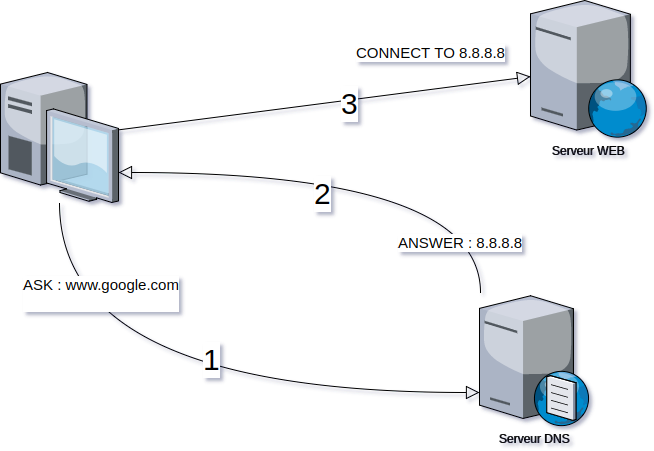
\includegraphics[width=300pt]{./cpp/Pictures/tp7+tp8-DNS}
  \caption{Résolution DNS}
  \label{Résolution DNS}
\end{figure}

La machine demande au serveur DNS l'adresse IP du nom de domaine \textit{google.fr} qui lui répond que l'adresse IP correspondante est \textit{8.8.8.8}, ainsi la machine pourra se connecter au serveur à l'adresse indiqué.

À l’aide du manuel, ainsi que la documentation de la fonction \mintinline{cpp}{gethostbyname()} permettant la translation d’un nom de domaine vers une adresse IP. J'ai créé un programme qui affiche les adresses IP des noms de domaine "www.yahoo.fr", "www.gmail.com" et "www.u-bourgogne.fr".

\inputminted[linenos,firstline=10,lastline=36]{cpp}{../sources/cpp/TP7-8/getHostByName.c}

%\subsection{Exercice 8 : Serveur multi-client en mode connecté}
